\chapter{Grundlagen\label{chap2:Zweites-Kapitel}}

Um eine Konzeption und eine prototypische Umsetzung einer Search Engine in \gls{mcc} zu ermöglichen wird in folgendem Kapitel auf die architekturellen Hintergründe von \gls{mcc} eingegangen. Hierfür werden zu Beginn allgemein gültige Architektur-Prinzipien erläutert, welche auch bei der Integration einer Search Engine berücksichtigt werden müssen und somit bei der Auswahl eines geeigneten Konzeptes von Bedeutung sind.

Aufbauend auf den Architektur-Prinzipien wird die verwendete Microservice-Architektur erläutert, wobei neben einer allgemeinen Einführung in die Architektur auch auf die Kommunikation von Microservices untereinander eingegangen wird. Um mögliche Fehlkonzeptionen zu vermeiden, werden häufig auftretende Anti-Pattern aufgezeigt, welche unter Umständen zu monolithischen Seiteneffekten führen könnten.

Abschließend wird anhand von verschiedenen modernen Informationssystemen die Funktionalitäten der Volltextsuche gezeigt. Neben den unterschiedlichsten Anwendungsfällen für eine Volltextsuche werden auch die technischen Besonderheiten von Search Engines vorgestellt.

\section{Software-Architekturen\label{sec2.1:Unterpunkt-1}}

\begin{quote}
    Die Software-Architektur eines Systems ist die Menge von Strukturen, die benötigt werden, um Entscheidungen über das System zu treffen, welche die Software-Elemente, die Relationen zwischen ihnen und die Eigenschaften von beiden betreffen. \textasciitilde{} Len Bass \cite{Bass.2013}
\end{quote}

Wie aus der Definition von Len Bass zu entnehmen ist, beschreibt eine Software-Architektur die Eigenschaften und Beziehungen von Software-Bausteinen zueinander \cite{Bass.2013}. Ein Software-Baustein wird hierbei als eine Teil-Komponente der gesamten Software betrachtet und wird bei der Erstellung einer Architektur als elementarer Bestandteil angesehen. Dabei wird ein Software-Baustein nicht näher spezifiziert, sondern als Komponente betrachtet, dessen konkrete Implementierung für die Architektur nicht von Bedeutung ist. Der Fokus einer Software-Architektur liegt auf den Schnittstellen der Software-Bausteine, über welche die Bausteine miteinander kommunizieren können.

\subsection{Architektur-Prinzipien\label{subsec2.1.1:Unterunterpunkt-1}}

Für das Erstellen einer guten Software-Architektur wurden von Vogel \cite{Vogel.2009} einige Grundprinzipien definiert. Diese Prinzipien sollten bei der Erstellung einer Software-Architektur beachtet werden: \cite{Vogel.2009}

\begin{description}
    \item[Lose Kopplung:]\hfill \\
    Der Kern einer Software-Architektur besteht aus der Beschreibung der Bausteine eines Software-Systems und deren Interaktionen zueinander. Unter dem Begriff Kopplung versteht man hierbei die Beziehung unter den Bausteinen einer Software-Architektur. Eine Kopplung charakterisiert demnach die Interaktionen der Bausteine.

    Eine starke Kopplung von Systembausteinen hat zur Folge, dass beim Verstehen und Ändern eines Bausteines auch zwingend weitere Bausteine verstanden und geändert werden müssen. Um jenes Problem zu umgehen, besagt das Prinzip der losen Kopplung, dass die Kopplung zwischen Systembausteinen möglichst niedrig gehalten werden sollen.

    Um eine lose Kopplung in einer Architektur zu erreichen, ist die Einführung von Schnittstellenabstraktionen ein wichtiger Aspekt. Dabei werden die Implementierungsinformationen hinter den Schnittstellen verborgen. Durch die Begrenzung von Schnittstellenelementen und der Häufigkeit des Austauschs der Schnittstellenelemente kann eine Kopplung von Systembausteinen kontrollierbar gemacht werden.

    \item[Hohe Kohäsion:]\hfill \\
    Im Gegensatz zur Kopplung, in welcher die Beziehungen zwischen Systembausteinen gemeint ist, versteht man unter dem Begriff Kohäsion die Abhängigkeiten innerhalb eines Systembausteins.

    Beim Prinzip der hohen Kohäsion ist das Ziel die Abhängigkeiten innerhalb eines Systembausteins möglichst hoch zu gestalten. Wie bei der losen Kopplung geht es auch hier um die lokale Änderbarkeit und Verstehbarkeit von Systembausteinen.
    
    Wie in \autoref{fig:kopplung_and_kohaesion} zu erkenne stehen Kopplung und Kohäsion normalerweise miteinander in einer Wechselbeziehung. Hierbei gilt, dass je höher die Kohäsion individueller Bausteine einer Architektur ist, desto geringer ist die Kopplung zwischen den Bausteinen. Schematisch ist dieser Zusammenhang in \autoref{fig:kopplung_and_kohaesion} abgebildet, worin zu erkennen ist, das eine Gesamtstruktur mit einer hohen Kohäsion und einer losen Kopplung (rechte Seite) eine höhere Übersichtlichkeit besitzt.

    \begin{figure}[H]
        \centering
        \includegraphics[width=0.7\linewidth]{images/Kopplung_und_Kohäsion.png}
        \caption{Zusammenspiel von loser Kopplung und hoher Kohäsion \cite{Vogel.2009}}
        \label{fig:kopplung_and_kohaesion}
    \end{figure}

    \item[Entwurf für Veränderung:]\hfill \\
    Durch den stetigen Wandel von Software-Systemen in Form von Anforderungen und Technologien, ist es von Vorteil solche Änderungen bereits in der Phase der architekturellen Konzeption zu berücksichtigen. Das Prinzip des Entwurfs für Veränderung (englisch: Design for Change) sieht nun vor, dass man vorhersehbare Änderungen architektonisch vorausplant. Dabei sollte man versuchen, die Architektur so zu entwerfen, dass man leicht mit den wahrscheinlichen Änderungen eines Software-Systems umgehen kann.

    \item[Separation of Concerns:]\hfill \\
    Abgeleitet von dem römischen Prinzip \glqq Teile und herrsche\grqq{} wird beim Prinzip Separation of Concerns ausgesagt, dass ein Software-System in individuelle Systembausteine zerlegt werden soll.

    Separation of Concerns unterstützt hierbei die Modularisierung eines Software-Systems. Es geht darum Teile eines Software-Systems zu identifizieren, welche für bestimmte Angelegenheiten, Aspekte und Aufgaben verantwortlich sind. Jene Teile werden dann als eigene Systembausteine gekapselt. Eine Zerteilung des Gesamtsystems in relativ unabhängige Einzelteile ermöglicht zudem noch die Verteilung von Verantwortlichkeiten für verschiedene Systembausteine und auch das parallele Arbeiten an dem Software-System durch mehrere Entwickler wird dadurch ermöglicht.

    Durch das Aufteilen des Software-Systems in relativ unabhängige Systembausteine werden auch die Prinzipien lose Kopplung und hohe Kohäsion begünstigt.

    \item[Information Hiding:]\hfill \\
    Das Prinzip Information Hiding sagt aus, dass man einem Klienten nur die für die Bearbeitung eines Problems notwendigen Informationen zeigen soll. Dies erleichtert die Gliederung und das Verständnis von komplexen Software-Systemen. Die restlichen Informationen sollen nach außen hin verborgen bleiben. Ermöglicht wird solch ein geheim halten von Informationen durch die Bereitstellung von definierten Schnittstellen, über welche nur bestimmte Informationen zu erreichen sind.

    \item[Abstraktion:]\hfill \\
    Als übergeordnetes Prinzip dient eine Abstraktion dazu, ein komplexes System verständlicher zu machen. Dazu werden wichtige Aspekte identifiziert und unwichtige Details vernachlässigt. Im Bereich der Software-Architektur gilt die Schnittstellenabstraktion als Teilprinzip der Abstraktion. Hierbei liegen die Schnittstellen im Fokus, welche für das Zustandekommen und die Qualität von Beziehungen verantwortlich sind.

    Solch eine Schnittstellenabstraktion in einem Software-System ist eng verbunden mit dem Prinzip der losen Kopplung und dem Information Hiding. Ein Aspekt für den starken Zusammenhang zwischen der Abstraktion und dem Information Hiding ist die Portabilität von Software-Systemen. So sollte eine Architektur oder ihre Systembausteine auch in anderen Umgebungen verwendbar sein. Um solch eine Plattformunabhängigkeit sicherzustellen, werden Abstraktionen verwendet, die ein Information Hiding der Platform-Details leisten.

    \item[Modularität:]\hfill \\
    Das Modularitätsprinzip, welches bereits auch in den Beschreibungen der anderen Prinzipien vorkam, definiert die Aufteilung eines Systems in klar definierte Bausteine mit abgegrenzten funktionalen Verantwortlichkeiten. Die Modularität ist dabei eine Kombination aus den Prinzipien Abstraktion, Separation of Concerns und Information Hiding, welche bei der Umsetzung der Prinzipien der losen Kopplung und der hohen Kohäsion kombiniert werden.

\end{description}

Auch für die spätere Konzeption einer Search Engine in einer Microservice-Architektur werden die eingeführten Prinzipien als Grundlage dienen.

\subsection{Monolithische und verteilte Architekturen\label{subsec2.1.2:Unterunterpunkt-2}}

Inhalt

\begin{figure}[H]
    \centering
    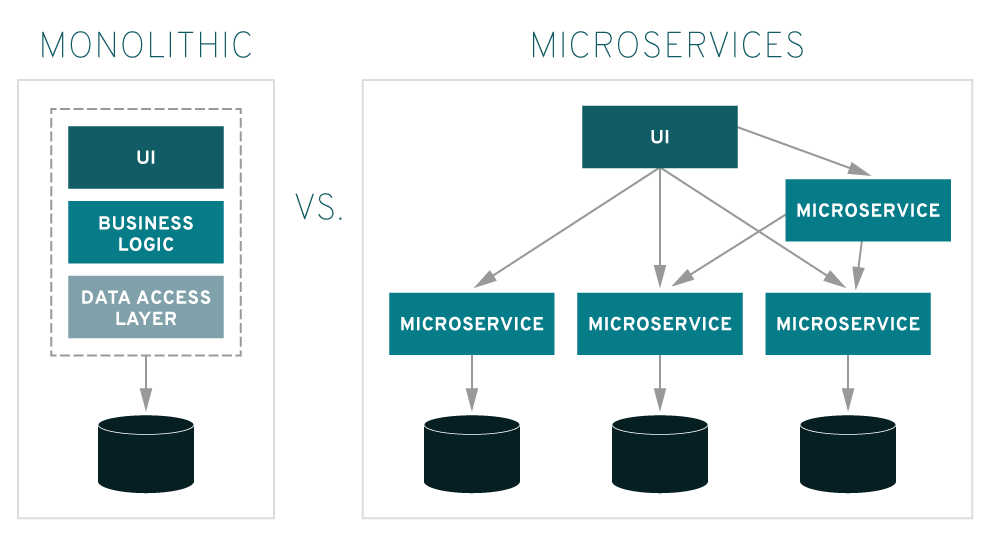
\includegraphics[width=0.7\linewidth]{images/monolithic-vs-microservices.png}
    \caption{3-Schichten-Architektur vs. Microservice-Architektur \cite{RedHatLimited.2021}}
    \label{fig:mono_vs_micro}
\end{figure}

\section{Microservice-Architektur\label{sec2.2:Unterpunkt-2}}

Für die Neugestaltung des \gls{mes} der Firma Enisco wird die Software auf einer verteilten Microservices-Architektur aufgebaut.

Die Kernelemente dieser Architektur sind die Microservices, welche der Modularisierung der Software dienen. Hierbei ist das unabhängige Deployment der Microservices eine wesentliche Eigenschaft. Die Möglichkeit Software modular aufzubauen, gibt es auch in monolithischen Architekturen. So helfen Ansätze, wie Klassen, Packages oder JARs in den Java-Umgebungen dafür eine Software in kleine Einheiten aufzuteilen und dadurch erweiterbar und wartbar zu machen. Das Problem ist jedoch, dass auch diese modularen Einheiten eine starke Abhängigkeit untereinander aufweisen und gemeinsam in einem Produktionsumfeld agieren müssen.

\subsection{Kommunikation zwischen Microservices\label{subsec2.2.1:Unterunterpunkt-1}}

Inhalt

\subsection{Vorteile\label{subsec2.2.2:Unterunterpunkt-2}}

Inhalt

\subsection{Microservice - Antipattern\label{subsec2.2.3:Unterunterpunkt-3}}

Inhalt

\section{Volltextsuche in modernen Informationssystemen\label{sec2.3:Unterpunkt-3}}

Inhalt

\subsection{Anwendungsfälle\label{subsec2.3.1:Unterunterpunkt-1}}

Inhalt

\subsection{Search Engines\label{subsec2.3.2:Unterunterpunkt-2}}

Inhalt